\section{Blurred images}
Detecting sharpness/blurriness of an image is a very central challenge in image quality assessment (IQA). Three different types of IQA-methods can be classified as:

\begin{itemize}
    \item Full reference\\
In this type of IQA, a reference image of perfect quality is given. This image will be distorted to varying degrees, and the goal is then to provide an algorithm, that can detect the degree of distortion.
    \item Reduced-reference\\
Here, a distorted version of the reference image is given together with a few informations on the perfect quality image. These informations can vary depending on the algorithm.
    \item No-reference\\
No reference image is given. Only an image of unknown quality. Again, the challenge is to provide an algorithm for determining the degree of distortion.
\end{itemize}

Detecting blur in this project, will be the no-reference challenge, as the final metric will be used live for detecting sharpness in the original image. This is considered the hardest problem of all three, and a perfect algorithm doesn't exist today.


\subsection{Description of algorithms}
In \cite{JNB} and \cite{FM}, a total of 16 different no-reference sharpness-metrics are mentioned. As a full test and implementation of all of them will be quite comprehensive, a few of them will be selected for testing. In table \ref{tab:blur_metrics} the metrics are listed in the first column. The parameters that the metrics are measured on are listed in the top row. They represent different methods used in construction of the algorithms and situations they might perform well in. The parameters can be described as follows:\\~\\
\textbf{Probability of blur-detection:}
Dividing the image into blocks. Using a formula on each block to determine the probability of the block being blurred...\\
\textbf{Edge detection:}
Using an algorithm - e.g. Canny or Sobel edge detector - for finding the edges in the image. The sharpness of the edges is often measured to estimate the sharpness of the image. \textcolor{red}{laplacian second order???}\\
\textbf{Training data:}
The metric contains constants, that are determined using a dataset.\\
\textbf{Different contents:}
The algorithm performed well in tests on determining sharpness of images containing different content.\\
\textbf{Fourier Transformation:}
The frequency domain of the image is used in determining its sharpness. Transforming an image into its frequency domain is quite computationally hard.\\
\textbf{Grayscale gradient:}
In the image, the gradients of the are calculated. These can be helpful in calculating edge thickness, and determining if there are sharp differences in the image. If there is much noise, using the gradient can unfortunately result in an estimation of an image being sharp even though the real motif isn't.\\
\textbf{Grayscale histogram:}
The normalized or un-normalized probability density function of the grayscale values of the image. As a completely blurred photo would approach a single gray color, and thus lose information, it is generally assumed, that sharper images tend to have more different grayscale values and not very many occurrences of each value, whereas more blurred images tend to have more middle grayscale values, and more occurrences of each value.\\
However, this is not always the case. E.g. one could easily have a sharp image with very dark and light gray values and almost none of the middle gray values.\\
As this assumption affects the accuracy of the sharpness-measure, one could assume, that this is the reason for the histogram-based metrics to be less popular.\\
\textbf{Grayscale variance:} Calculated as the variance over the whole grayscale image. As the image becomes more blurred, the grayscale values will become more similar, thus decreasing the variance.\\
\textbf{Noise robust:}
The correctness of the sharpness measure generally is not affected by noise.\\

For all of the algorithms, it is noted whether they perform good in the situation or use the concerned method.
\setlength\LTleft{-3cm}\begin{longtable}{|| p{.16\textwidth} || p{.13\textwidth} | p{.08\textwidth} | p{.1\textwidth} | p{.1\textwidth} | p{.1\textwidth} | p{.11\textwidth} | p{.11\textwidth} | p{.11\textwidth} | p{.09\textwidth} ||}\hline
    Sharpness metric & Probability of blur-detection 
        & Edge detection & Training data & Different contents & Fourier Transformation & Grayscale gradient & Grayscale histogram & Grayscale variance & Noise robust \\\hline\hline
    \textbf{Variance}\cite{jnbm05} 1982                                & %Variance of whole grayscale. (variance is close to contrast). robust to noise 
        no & no & no & no & no & no & no & \textbf{yes} & \textbf{yes} \\\hline
    Auto-correlation-based\cite{jnbm06}, 2000                  & %Autocorrelation-function (Fourier transformation) 
        no & no & no & no & \textbf{yes} & no & no & no & ok \\\hline
    \textbf{Derivative-based}\cite{jnbm06}, 2000 \textcolor{red}{laplacian}                     & %Gradient. Noise sensitive. 
        no & no & no & no & no & \textbf{yes} & no & no & no \\\hline
    Perceptual blur\cite{jnbm07}, 2004                       & %Edge detection. "very low computational complexity" 
        no & \textbf{yes} & no & no & no & no & no & no & ok \\\hline
    Frequency threshold\cite{jnbm08} &
    no & & no & no &  &  & &  & \\\hline
    Kurtosis\cite{jnbm09}\cite{jnbm10}, 2004**             & 
        no & \textbf{yes} & no & no & \textbf{yes} & no & no & no & no/ok\\\hline
    Histogram threshold\cite{jnbm08}, 1991 & %"assumed that a sharper image contains a higher number of grayscale levels" 
        no & no & no & no & no & no & \textbf{yes} & no & ok \\\hline
    Histogram entropy-based\cite{jnbm11}, 2001 & %higher entropy of grayscale levels = sharper image 
        no & no & no & no & no & no & \textbf{yes} & no & ok \\\hline
    \textbf{Histogram frequency-based}\cite{jnbm12}, 1999 & %"minimal computational load" cam perform robust sharpness detection on videos. Probably fast.
        no & no & no & no & (\textbf{yes}\footnote{The images need to be in JPEG or MPEG compressed format. That is, the DCT (Fourier-related transform) has to be calculated before applying the algorithm.}) & no & no & no & ok \\\hline
    Shaked-Tastl\cite{jnbm13}, 2005 & %"is computationally efficient, and requires fewer computations than a 3x3 convolution", "correlates well with perceived sharpness, and is to a large degree invariant to image content". Is feature-based (no special features in our dataset - however they use edges) 
        no & \textbf{yes} & no & ok & no\footnote{\textit{we use spatial filters rather than a full 2D Fourier transform}\cite{jnbm13}} & \textbf{yes} & no & (no) & ok \\\hline
    Image Quality Measure\cite{jnbm14}, 1992 & %Using Fourier transformation (computationally hard). Power spectra (ft of autocorrelation function). Determining less sharpness for images with large smooth areas. This could be ok, since it is enough that it can determine sharpness according to a threshold. 
        no & no & no & ok & \textbf{yes} & no & no & no & ok \\\hline
    Noise Immune Sharpness\cite{jnbm03}\cite{jnbm07}, 2005 & % Performing well on noisy images. Using Perceptual blur metric.
        no & \textbf{yes} & no & no & no & no & no & no & \textbf{yes} \\\hline
    \textbf{No-reference Blur}\cite{jnbm17}, 2003 & %Parameters are estimated by training on a dataset. Gradient. Blur is detected by calculating edge widths in gradient dir.
        no & \textbf{yes} & \textbf{yes} & no & no & no & no & no & no \\\hline
    Just Noticeable Blur\cite{JNB}, 2009 & %Probability summation. 
        \textbf{yes} & \textbf{yes} & no & \textbf{yes} & no & no & no & no & ok \\\hline
    CPBD\footnote{Cumulative probability of blur detection}\cite{CPBD}, 2010 & 
        \textbf{yes} & \textbf{yes} & no\footnote{Training data is used to determine the discrete quality classes, but not the continuous scores of the metric.} & \textbf{yes} & no & no & no & no & ok \\\hline
    \textbf{Frequency Domain}\cite{FM}, 2013 & %Good at gaussian blur and motion blur. Frequency domain. 
        no & no & no & \textbf{yes} & \textbf{yes} & no & no & no & ok \\\hline %O(nlogn) 
    \caption{Different no-reference metrics for detecting blur in an image, what methods they use and what situations they perform well in.} \label{tab:blur_metrics}
\end{longtable}

% In table \ref{tab:blur_metrics} the methods of the blur-metrics mentioned in article \cite{JNB} and \cite{FM} have been listed. To make the best possible solution to the blur-detection on the time given, a few metrics will be chosen to be tested and compared to each other.

% It is assessed that it is not important that the metric is good at noise detection and correctly determining blur of images with different content, as all the relevant images in this project will contain very similar motifs, photographed using the same instrument.\\
% With this thought in mind, a group of metrics using different methods and performing good in different situations, are chosen for this challenge. However, as the images are expected to be very alike, both methods using training data sets (No-reference Blur Metric, CPBD) are chosen to be tested.\\
% - The Histogram threshold metric will not be included: an assumption is made, \textit{assumed that a sharper image contains a higher number of grayscale levels}\cite{JNB}, and in the tests\cite{JNB} it does not perform well on any of the data sets.\\
% - JNB is using probability summation and edge detection and is good for different contents - looks the same as CPBD except for the training data.\\
% - According to \cite{FM}, FM should outperform both JNB and CPBD on determining image sharpness correctly on images with different content. However, the best metric to measure on images of different content is probably not needed.\\
% - IQA vs. Autocorrelation-based. Choose at most one. Choosing none, as they both use Fourier-transform (Autocorrelation-function): Histogram frequency-based is exploiting that the image fft is already calculated...\\


% Generally sharpness-measures using the grayscale histogram of the image are less popular\cite{JNB} and perform worse than measures using other measures on i.a. optical microscopy images of tissue\cite{jnbm08}

The following sharpness-metrics will be gone forward with: Variance, Derivative-based, Histogram frequency-based, No-reference blur and Frequency domain. The first one, variance, is a very simple metric, that will be included to create a good baseline to compare performance and accuracy of the other metrics included. The derivative-based and frequency domain are some classical methods\cite{} and are therefore included. The no-reference blur-metric is included as it uses a training dataset, and as the images are all of ear canals, it would be very interesting to see if this metric has better accuracy. The last one, histogram frequency-based metric, is included, as it is developed to function well on MPEG (movie) images, and therefore might evaluate the images very quickly without compromising on accuracy.\\
These metrics will be tested using a few different test-methods: sensitivity/specificity. Accuracy, f-score. Area under the roc...\\
\textit{Sklearn\footnote{\url{https://scikit-learn.org/stable/modules/model_evaluation.html}}} has implementations of these tests, that will be used in the project.\\
When testing, it will be assessed whether a few of the metrics should be used together in the final program, as they might perform better that way.



\subsubsection{Analysis of running time}

\subsubsection{Cumulative probability of blur detection}
% What is JNB and JND?
The used implementation of the CPBD metric\cite{code_CPBD} is based on the concept of JNB defined in \cite{JBN}. JNB is explained: \textit{The "just noticeable blur" (JNB) is the minimum amount of perceived blurriness around an edge given a contrast higher than the JND}\cite{JNB}, where JND is the just noticeable difference \textit{the JND is the minimum amount by which a stimulus intensity must be changed relative to a background intensity in order to produce a noticeable variation in sensory experience}\cite{JNB}. The JNB have been experimentally determined in relation to the contrast in an image.

The metric starts out by splitting the input image into blocks of $64\cdot 64$ pixels. Canny edge detection by \textit{sci-kit\footnote{\url{https://scikit-image.org/docs/dev/api/skimage.feature.html\#canny}, accessed October 5, 2021}} is used on the whole image to classify the blocks as edge or non-edge blocks.

\textbf{The canny edge detector}\footnote{\url{https://scikit-image.org/docs/dev/api/skimage.feature.html}, accessed October 4, 2021} takes as input the output of the \textbf{sobel edge detector}, which works by applying a 2-dimensional Gaussian filter with $\sigma=1$ to the image to smooth out noise\footnote{\url{https://scikit-image.org/docs/dev/api/skimage.filters.html?highlight=gaussian\%20filter\#skimage.filters.gaussian}, accessed October 4, 2021}. The Gaussian filter is applied first in one direction and afterwards in the other\footnote{\url{https://github.com/scipy/scipy/blob/9492369e7f76c8206ac1c375e75375ca7410a7e7/scipy/ndimage/filters.py}, accessed October 7, 2021}. This takes $O(w_g \cdot N \cdot M + h_g \cdot N \cdot M)$\footnote{\textcolor{red}{depends on 1D+1D or 2D. It is 1D+1D}}, where $w_g$ and $h_g$ are respectively the width and height of the Gaussian filter.\\
After this, the horizontal and vertical sobel filter 
$$sobel_h =
\begin{bmatrix}
 1 &  2 &  1\\
 0 &  0 &  0\\
-1 & -2 & -1
\end{bmatrix}$$
$$sobel_v = 
\begin{bmatrix}
 1 &  0 & -1\\
 2 &  0 & -2\\
 1 &  0 & -1
\end{bmatrix}
% \begin{bmatrix}
%  2 &  2 &  0\\
%  2 &  0 & -2\\
%  0 & -2 & -2
% \end{bmatrix}
$$
are applied to all the pixels in the image, that is $O(N\cdot M)$.
% Apply the horizontal and vertical Sobel operators to get the gradients within the image. The edge strength is the norm of the gradient.
Now the canny edge detector can thin out the edges to be 1 pixel wide. This requires going through all found edges, which in the worst case is $O(N\cdot M)$ edge pixels. To thin the edges, each edge point will be traversed a constant number of times, $c$: first to sort the edges into horizontal, vertical and diagonal edges, and then compare their values to the reversed and normals to see if they are greater in those directions. The points for the edges are picked using interpolation. All of this takes $O(c\cdot N\cdot M) = O(N\cdot M)$ time.

Lastly in the canny edge detector, a hysteresis thresholding is performed, where all the edge pixels below a low threshold are discarded, and all the edge pixels above a high threshold are included. Edge pixels that are 8-connected to the high threshold edges, are included in the final edges as well to store as much relevant information as possible. This can be implemented in $O(N\cdot M log N\cdot M)$ time according to
\footnote{\url{https://stackoverflow.com/questions/17458237/time-complexity-of-canny-edge-detector\#:~:text=The\%20final\%20step\%20works\%20by,O(mn\%20log\%20mn)}, accessed October 5, 2021. \textcolor{red}{examine this closer}}. Thus, the total running time of canny will be $O(N\cdot M log N\cdot M)$.\\

In the article\cite{CPBD}, now would be the time where the edge pixels were counted, and the smooth blocks were discarded. However, the implementation\cite{code_CPBD} will at this time \textbf{compute the edge widths}, $w(e_i)$, instead. This is done using the sobel edge detector\cite{code_CPBD} described earlier, as the edges in the canny edge detector have been reduced to a width of 1 pixel. In the implementation, all $w(e_i)$ are calculated in $O(N\cdot M\cdot 101)=O(N\cdot M)$. This includes calculating the gradients of the image, $O(N\cdot M)$. The angles of the edges calculated in $O(N\cdot M)$. The angles are used for calculating edge widths in $O(N\cdot M\cdot 3\cdot 101)=O(N\cdot M)$.

Next step in the implementation is to loop over all the $\dfrac{N\cdot M}{64}$ blocks in the image. Here, the edge pixels are counted, and a threshold of $t=0.2\%$ is now used to determine if the block is an edge-block. That is, if the number of edge pixels in the image detected by the canny edge detector is above 0.2\% of all the pixels in the block, the block is considered an edge block, and otherwise as a smooth block. The counting requires looking at every pixel in the block, that is $block\_size=64^2$.

If the block is considered an edge block, the \textbf{JNB edge width}, $w_{JNB}(e_i)$, is determined by calculating the block contrast $C=max(grayvalue)-min(grayvalue)$ and from this determining the JNB as in \cite{JNB} from the experiments mentioned earlier. Finding the grayscale values for the contrast takes $O(64^2)$ time.

Now, the \textbf{probability of blur detection} for each edge $e_i$ can be computed. This is done using the following equation 
$$P_{BLUR}=P(e_i)=1-e^{-\lvert\dfrac{w(e_i)}{w_{JNB}(e_i)}|^\beta}$$
mentioned in \cite{CPBD} and explained in \cite{JNB}, where $\beta = 3.6$.

The probability distribution function of $P_{BLUR}$ is updated in $O(64^2)$ time, as the last step in the loop on the blocks.

The final step of the metric is to \textbf{calculate the CPBD}. The equation from \cite{CPBD}
$$CPBD = P(P_{BLUR} \leq P_{JNB}) = \sum_{P_{BLUR}=0}^{P_{BLUR}=P_{JNB}} P(P_{BLUR})$$
is used, where $P(P_{BLUR})$ is the value of the pdf of a given $P_{BLUR}$. Only the first 64\% of the pdf are summed, as \textit{It should be noted that when $w(e_i) = w_{JNB}(e_i)$ then $P_{BLUR} = 63\% = P_{JNB}$}.\cite{CPBD}

This will provide a total time complexity of 
$$O(canny + sobel + |blocks| \cdot (count\_edge\_pixels + contrast + update\_pdf) + sum)$$
$$= O((N\cdot M log N\cdot M) + (N\cdot M) + \dfrac{N\cdot M}{64} \cdot (3\cdot 64^2) + 64)$$
$$= O(N\cdot M log N\cdot M)$$


\subsubsection{Histogram frequency-based metric}
The Histogram frequency-based metric\cite{jnbm12} bases its solution on images and videos in the file format of JPEG and MPEG, as it is estimated that the compression of the images can be exploited for fast and effective blur detection. The implementation used\cite{code_HF} is implemented in \texttt{C}.

% \textit{In this paper, we present a new solution proposed
% to aim at exploiting the available DCT information in
% MPEG or JPEG compressed video or images while involving a minimal computational load. As presented in the next section, the technique is based on histograms
% of non-zero DCT occurrences, computed directly from MPEG or JPEG compressed images.}\cite{jnbm12}


\textbf{The JPEG format} compresses images\cite{jpg} by i.a. applying the DCT\footnote{discrete cosine transform} to $8\times 8$ blocks of the image.

\textcolor{red}{DCT: should the formula be included?}

The output of the DCT is a matrix, where the top left cell is called the DC\footnote{constant component}, as it does not depend on the index, as $x=0 \text{ and } y=0$. The remaining 63 cells are the AC\footnote{alternating component \textcolor{red}{(add more detail?)}} cells.
%The DC describes \textcolor{red}{\textit{the basic hue for the entire} $8\times 8$ block}.
Precisely this DCT computation is what is exploited in the metric, as \textit{The DCT coefficients used within MPEG are intended for compression and are deeply related to the image content. Basically, they reflect the frequency distribution of an image block}\cite{jnbm12}. It is also known from i.a. \cite{FM}\footnote{\textit{when the blur in an image increases the number of high frequency component in the images decreases}} that there is a connection between frequency and blurriness of an image. In the histogram frequency metric this is used by looking at the absence of high AC coefficients.

In the implementation\cite{code_HF} a histogram (an array of length 64) is initialized to all 0's. Then all $8^2$ luminance blocks\footnote{\textcolor{red}{explain}} in the image are traversed and the DCT values that are greater than a threshold \textit{minDCTValue} are inserted into the histogram by adding a 1 to that index. The \textit{minDCTValue} threshold is used for filtering away image noise. All DCT values below this threshold remains 0 in the histogram.\\
After this, all the values of the histogram will be reviewed using another threshold, \textit{maxHistValue}. If \texttt{histogram\_value < maxHistValue $\cdot$ histogram\_first\_value} the histogram bucket will be discarded, otherwise its weight of a wheighting grid defined in \cite{jnbm12} will be added to $blur$, initialized to 0. The final metric is calculated by
$$HF=1-\dfrac{blur}{weight\_total}$$
where $weight\_total$ is the sum of all weights in the weighting grid. A lower result would mean a more blurred image, while a greater result would mean a sharper image.
%This grid weights diagonal DCT coefficients higher to better represent global \textcolor{red}{blur}.
% \textit{ 0\% would mean that the frame is totally blurred while 100\% would mean that no blur at all is present in that particular frame}

This gives a time complexity of $O(\dfrac{N\times M}{8}\cdot 64 + 64) = O(N\cdot M)$.

%\textbf{Luminance and chrominance}\\
%Colors of the image are converted from RGB or Cy, Ma, Ye (and bk) into three components space luminance (Y) and chrominance (Cr, Cb) signals.

%\textbf{Loop: all macroblocks} only luminance is being used in the implementation \cite{code_HF}.
%\hspace{.5cm}\textbf{Loop: every luminance block}\\
%    $O(\dfrac{N\cdot M}{8})=O(N\cdot M)$\\

In the article\cite{jnbm12} the metric also loops over all macroblocks\footnote{\textcolor{red}{explain}}. However, this has been excluded in the implementation\cite{code_HF}.


\subsubsection{Frequency Domain Image Blur Measure}
The FM metric is based on the observation that \textit{when the blur in an image increases the number of high frequency component in the images
decreases}\cite{FM}. Thus, the metric works by transforming the image into frequency domain and calculating the no. high frequency components in the image above a threshold. This number is then used to evaluate the sharpness of the image. The sharper the image, the higher the score.

In the implementation\cite{code_FM} the Fast Fourier Transform (FFT) is calculated on the input image. This takes $O(N\cdot M log N\cdot M)$\cite{FM}, which is also the total time complexity of FM. Then the FFT is shifted so the 0-frequency is centered in $O(N\cdot M)$ time. The maximum, $M$, of the absolute value of all Fourier coefficients are calculated $M=max(AF)$, also in $O(N\cdot M)$ time, where $AF=|centered\_Fourier|$.

The final quality assessment is calculated as
$$FM=\dfrac{T_H}{M\cdot N}$$
where $T_H=|AF > t|$ and $t = M/1000$ is the mentioned threshold.


\subsubsection{Variance of the Laplacian}
This metric is implemented in python\cite{code_LV} and based on a blogpost\footnote{\url{https://www.pyimagesearch.com/2015/09/07/blur-detection-with-opencv/}, accessed: October 4, 2021} referring to an article\footnote{\url{https://decsai.ugr.es/vip/files/conferences/Autofocusing2000.pdf}, accessed: October 4, 2021} from 2000. The idea is, that taking the laplacian of an image will leave the edges in the image visible. Calculating the variance of the laplacian image will provide a score, that can be compared to an experimentally set threshold. If the score is below the threshold, the image is blurred and vice versa. The threshold may vary considerably depending on the image data set.

If the image contains colors, that is, it is stored in 3 dimentions, it is initially converted to grayscale. This takes $O(N\cdot M)$ where $N$ and $M$ are respectively the horizontal and vertical no. pixels in the image. After this, the laplacian filter\cite{code_LV}:
$$laplacian\_filter = 
\begin{bmatrix}
0 &  1 & 0\\
1 & -4 & 1\\
0 &  1 & 0
\end{bmatrix}$$
is applied to the original image. This is also applied to all pixels in the image, and thus takes $O(N\cdot M)$ time. Next the variance:
$$\sigma^2 = mean(|a - mean(a)|^2)$$
where 
$$mean(x) = \dfrac{\sum {x}}{|x|}$$
is applied on all the laplacian values. Thus, the time complexity of $\sigma^2$ is $O(N\cdot M)$. Finally the variance is compared to the threshold, $O(1)$. The complete time complexity of the metric is thus $$O(N\cdot M) + O(N\cdot M) + O(N\cdot M) + O(1) = O(3N\cdot 3M) = O(N\cdot M)$$


\subsection{Performance tests}\label{Performance tests}
In the classification of sharpness of the otoscopic images of the eardrum, it is more important that no blurry images are classified as sharp than that sharp images are classified as blurry, as the goal is to create a dataset consisting of good images. In order to examine the performance of the implemented blur-metrics, the following test methods will be used.

\subsubsection{Confusion matrix}
The confusion matrix displays the correctness of the output of a classifier given a binary ground truth. There are four output possibilities: 
\begin{enumerate}
    \item True positive, \textbf{TP}: when a positive output is also positive in the ground truth.
    \item True negative, \textbf{TN}: when a negative output is also negative in the ground truth.
    \item False positive, \textbf{FP}: when a ground true negative element is classified as positive.
    \item False negative, \textbf{FN}: when a ground true positive element is classified as negative.
\end{enumerate}
The confusion matrix contains the sum of these different outputs in a matrix as:
\begin{table}[h!]\begin{tabular}{|c||c|c|}\hline
Ground true negatives & TN & FP\\\hline
Ground true positives & FN & TP\\\hline\hline
& predicted as false & predicted as true\\\hline
\end{tabular}\end{table}\\
This is also defined in \cite{img_analysis}\footnote{chapter 7.4.3} and \cite{ML_book}\footnote{chapter 16.2.1}. The output of the classifier is in our case continuous, thus a threshold is needed to determine a binary output. A good approach to determining a threshold is using the ROC curve.


\subsubsection{Area under the ROC curve}
As the ground true classes may vary in size, the classes are normalized to provide a valid starting point to choose a threshold from. The normalized values are called the true positive rate (TPR also known as sensitivity) and the false positive rate (FPR, also known as probability of false alarm) defined as:
\begin{equation}
    sensitivity = TPR = \dfrac{TP}{TP+FN}
\end{equation}\label{TPR}
and
\begin{equation}
    FPR = \dfrac{FP}{FP+TN}
\end{equation}\label{FPR}
as in \cite{ML_book}\footnote{chapter 16.2.1}.
The receiver operating characteristic curve (ROC curve) is a curve describing the TPR on the y-axis and the FPR on the x-axis given a varying threshold. Labeling all outputs of the classifier above a threshold $t$ as positive and vice versa, choosing a threshold $t$ that is less than all the outputs of the classifier, will provide only positive outputs, thus providing a TPR and FPR of 1. On the other hand, a $t$ greater than all outputs will provide a TPR and FPR of 0. Assuming that the classifier is better than random, thus generally classifying the inputs as negative when negative and vice versa, the area beneath the ROC curve will be between 0.5 and 1. This is because, if the inputs are classified as described, increasing $t$ it will move over the negative labeled outputs faster than the positive labeled outputs.\textcolor{red}{insert diagrams}

Knowing this, the area under the curve (AUC), can be calculated as the integral of the ROC curve and used for measuring performance. If the ROC curve goes through $(0,1)$, the AUC will be equal to 1, and the TPR and FPR will be respectively 1 and 0, thus all the true positives will be labeled as so, and there will be no false positives. If, however the AUC equals $0.5$, this will indicate that the ROC in average lies on the straight line between $(0,0) \text{ and } (1,1)$. If the ROC goes through $(0.5,0.5)$, the TPR and FPR will be equal to $0.5$, and thus the classifier will perform as good as a random classifier.


\subsubsection{Sensitivity / specificity}
Sensitivity has already been defined in equation \ref{TPR}. This is a measure on how many positives are classified as positives compared to the ground truth number of positives. The specificity (TNR, true negative rate) is defined as the normalised true negatives:
\begin{equation}
    specificity = TNR = \dfrac{TN}{TN+FP}
\end{equation}
In the case of evaluating sharp otoscopic images, this measure is not as important, as mentioned in \ref{Performance tests}. However, it still provides a good measure of how well the metric tend to perform.


\subsubsection{Accuracy}
The accuracy of the metric is defined as
$$accuracy = ACC = \dfrac{TP+TN}{TP+FP + TN+FN}$$
That is, it is a measure of how many inputs are correctly classified compared to the total number of inputs.

\subsubsection{F1-score}
The precision (positive predictive value (PPV)) is calculated as
$$precision = PPV = \dfrac{TP}{TP + FP}$$
This is a measure on how precise the positive outputs of the classifier are, which in this case is a very important measure, as it describes the false positives, that, as explained, are the results that should be minimized.

$F_1$-score is defined as the harmonic mean of sensitivity and precision. That is:
$$F_1 = \dfrac{2}{PPV^{-1} + TPR^{-1}} = 2\dfrac{PPV\cdot TPR}{PPV + TPR} = \dfrac{2TP}{2TP+FP+FN}$$
This is another way to measure the accuracy of a binary classifier, though without including the true negatives. The score will be between 0 and 1. 0 if either PPV, TPR or both are 0, and 1 if PPV and TPR are both 1, that is they classify perfectly compared to the ground truth.\footnote{\textcolor{red}{Both equations need a source}}



\subsection{Generation of synthetic dataset}
To extend the image data, the images have been mirrored and a Gaussian filter has been applied to the sharp images.\\

\subsubsection{Rotate...}
insert images

\subsubsection{Gaussian filter}

To the sharp original and mirrored images, a Gaussian filter (described in \cite{img_analysis}\footnote{chapter 5.2} with a kernel size of $15\times15$ and different values of $\sigma$ have been applied.

\begin{figure}[H]
    \centering
    \begin{subfigure}[t]{0.3\textwidth}
        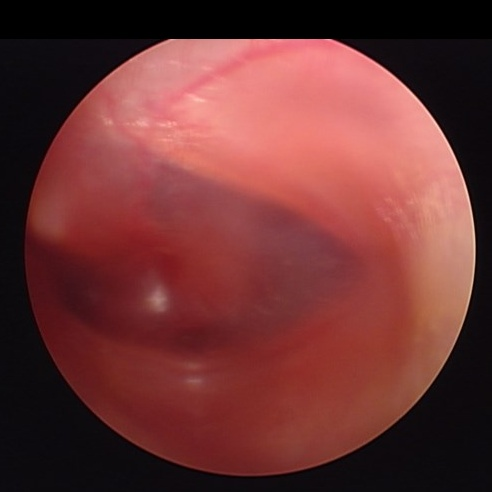
\includegraphics[width=\textwidth]{Figures/BlurredImages/Gaussian/21.png}
        \caption{Naturally blurred image for comparison with the synthetically blurred images.}
        \label{fig:blur}
    \end{subfigure}\hspace{1em}
    \begin{subfigure}[t]{0.3\textwidth}
        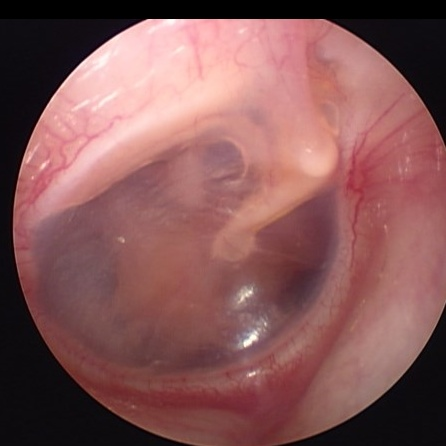
\includegraphics[width=\textwidth]{Figures/BlurredImages/Gaussian/13.png}
        \caption{A natural image with no problems.}
        \label{fig:sharp}
    \end{subfigure}\hspace{1em}
    \begin{subfigure}[t]{0.3\textwidth}
        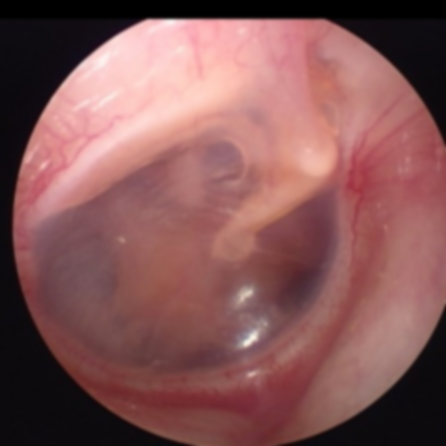
\includegraphics[width=\textwidth]{Figures/BlurredImages/Gaussian/60.png}
        \caption{The sharp image (\ref{fig:sharp}) with applied Gaussian filter with $\sigma=1.5$.}
        \label{fig:blur_synth_1.5}
    \end{subfigure}
    
    \begin{subfigure}[t]{0.3\textwidth}
        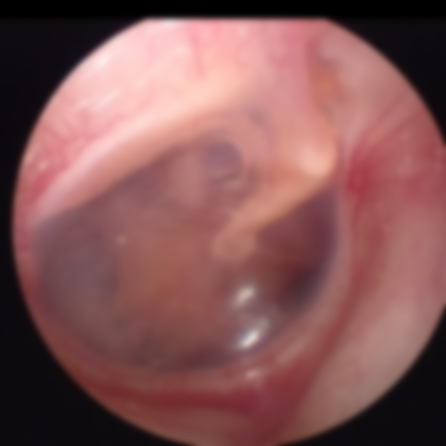
\includegraphics[width=\textwidth]{Figures/BlurredImages/Gaussian/128.png}
        \caption{\ref{fig:sharp} blurred with $\sigma = 3$.}
        \label{fig:synth_blur_3}
    \end{subfigure}\hspace{1em}
    \begin{subfigure}[t]{0.3\textwidth}
        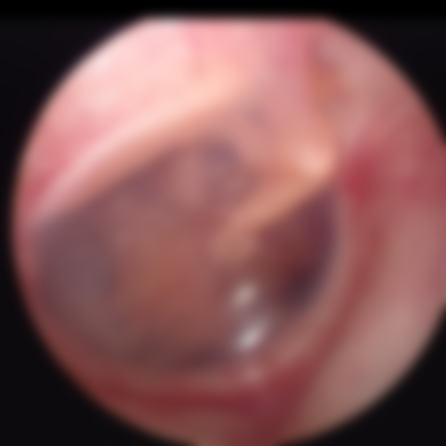
\includegraphics[width=\textwidth]{Figures/BlurredImages/Gaussian/196.png}
        \caption{\ref{fig:sharp} blurred with $\sigma = 6$.}
        \label{fig:blur_synth_6}
    \end{subfigure}
\end{figure}




\subsection{Results}
The continuous CPBD metric\cite{CPBD}, the Histogram frequency-based metric (HF) and the FM metric have been evaluated on the original dataset. They all output a score in the interval $[0,1]$. The implementations of the CPBD and FM metric are both in python, while HF is implemented in \texttt{C}. This likely has a thing to say in how fast the algorithms run.

\begin{figure}[H]
    \centering
    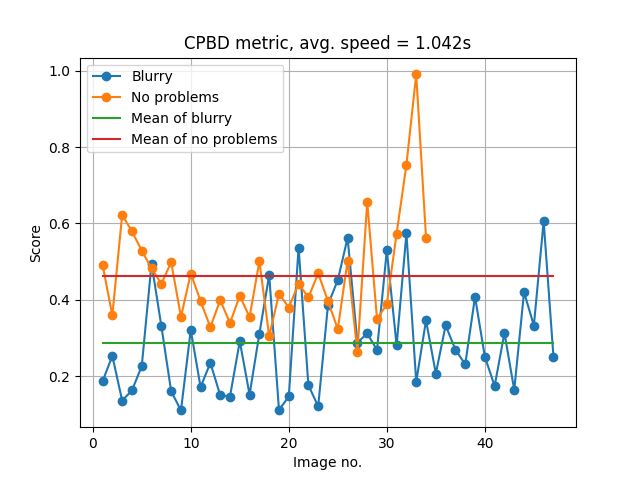
\includegraphics[width=.8\textwidth]{Figures/BlurredImages/output_cpbd.png}
    \caption{Results of running CPBD on the blurry and the good images.}
    \label{fig:cpbd}
\end{figure}
Figure \ref{fig:cpbd} displays the performance of the CPBD-metric. Fortunately, as can be seen on the graph, the blurry images tend to have lower score than the images without problems. The average time on evaluating an image is $1025.95\si{ms}$, calculated as $\texttt{avg.speed}=\dfrac{sum(time)}{no\_images}$, which is quite slow. However, one second might not be too slow when interactively evaluating a single image at a time.

\begin{figure}[H]
    \centering
    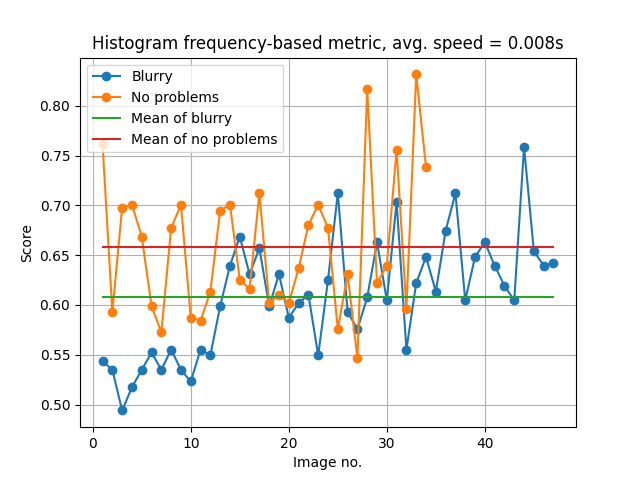
\includegraphics[width=.8\textwidth]{Figures/BlurredImages/output_HF.png}
    \caption{$\texttt{avg.speed} = \dfrac{0.306\si{s}}{47+34} \approx 0.008\si{s}$. The sharper the image, the lower the metric is. Since the metric is measured in percentage and thus lies between 0 and 1, the output has been normalized so that the output is still between 0 and 1, but the sharper images will have lower score. It is normalized by the simple $\texttt{norm}=1-\texttt{result}$.}
    \label{fig:HF}
\end{figure}
As can be seen in figure \ref{fig:HF}, the HF metric immediately seems to perform reasonably well, but not as good as CPBD. There is only about $0.66-0.61=0.05$ between the two means in HF, whereas in CPBD there is about $0.48-0.3=0.18$. However, the speed of this metric is much lower, $0.008\si{s}$ pr. image than the $1\si{s}$ from CPBD.

\begin{figure}[H]
    \centering
    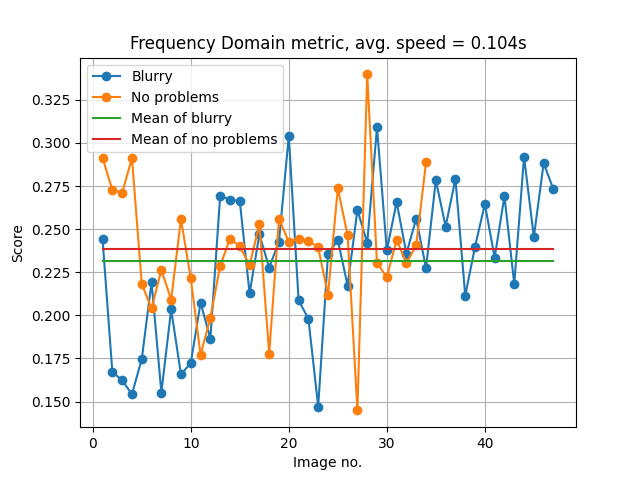
\includegraphics[width=.8\textwidth]{Figures/BlurredImages/output_FM.png}
    \caption{$\texttt{avg.speed} = \dfrac{4.694\si{s}+3.690\si{s}}{47+34} \approx 0.104\si{s}$. The sharper the image, the higher the metric.}
    \label{fig:FM}
\end{figure}
The initial impression of figure \ref{fig:FM} is that the results are almost random. The distance between the two means is around $0.240-0.232=0.008$, which is much lower than the distance in both the HF metric and the CPBD metric.\\

To enable binary evaluation of an image, the two means of respectively figure \ref{fig:cpbd}, \ref{fig:HF} and \ref{fig:FM} are used to determine a threshold. The threshold is calculated as $threshold=min(mean1, mean2) + |\dfrac{mean1-mean2}{2}|$ to account for the different amount of sharp and blurry images in the dataset. Scores above the threshold will be evaluated as sharp and vice versa.

\begin{figure}[H]
    \centering
    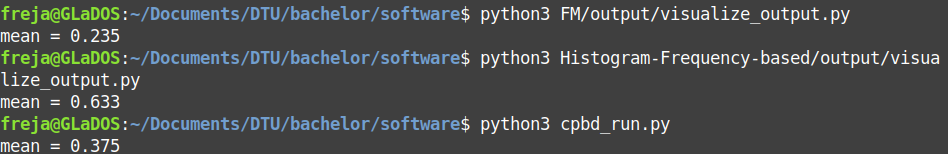
\includegraphics[width=\textwidth]{Figures/BlurredImages/means.png}
    \caption{The mean values (thresholds) of all the results from the metrics in order Frequency Domain\ref{fig:FM}, Histogram frequency-based\ref{fig:HF} and CPBD\ref{fig:cpbd}}
    \label{fig:means}
\end{figure}
These means will be used as thresholds to provide a binary measure of the images: if the image lies above the threshold, it will be classified as sharp and vice versa.\\

The classification into sharp and blurry images by the three metrics are plotted in confusion matrices and area under the ROC curves. In the confusion matrix, the true positives in the top left corner are the ground true sharp images evaluated as sharp by the metric. The lower right square represents the true negatives, that is the number of ground true blurry images evaluated as blurry. False positive and false negative are contained in respectively the lower left and the top right.\\ % lav matrix i teoriafsnit om testmetoder

\begin{figure}[H]
    \centering
    \begin{subfigure}[t]{0.49\textwidth}
        \centering
        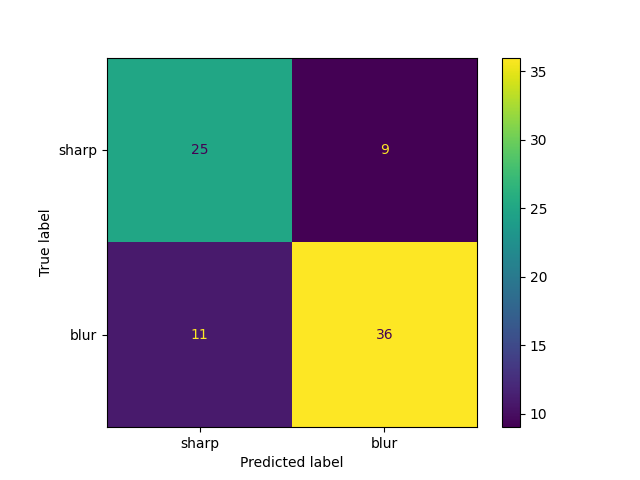
\includegraphics[width=\textwidth]{Figures/BlurredImages/output_cpbd_conf_mat.png}
        \caption{Confusion matrix of CPBD results. The true positive and true negatives make up the majority of the results.}
        \label{fig:hf_conf_mat}
    \end{subfigure}
    \hfill
    \begin{subfigure}[t]{0.49\textwidth}
        \centering
        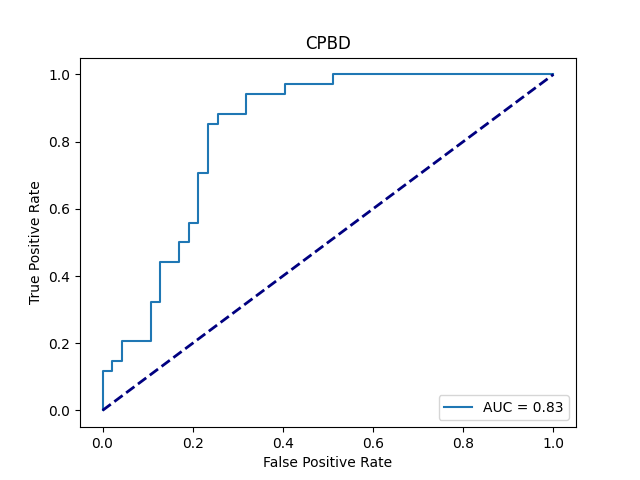
\includegraphics[width=\textwidth]{Figures/BlurredImages/output_cpbd_roc.png}
        \caption{The AUC of CPBD has a score of 0.83. This is a quite good result.}
        \label{fig:hf_roc}
    \end{subfigure}
    \begin{subfigure}[t]{0.49\textwidth}
        \centering
        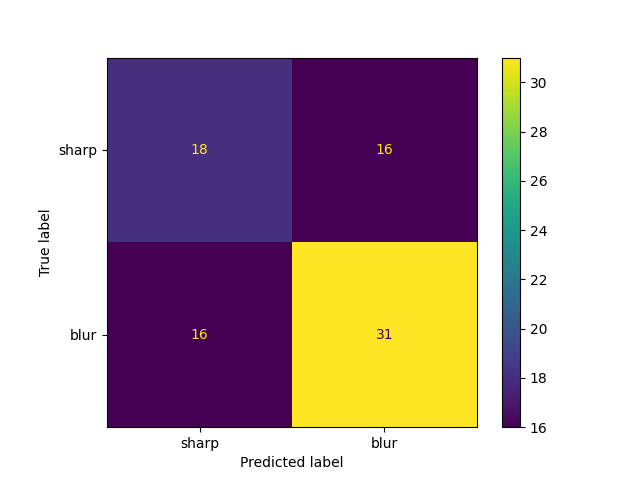
\includegraphics[width=\textwidth]{Figures/BlurredImages/output_HF_conf_mat.png}
        \caption{Most of the results from the HF metric lies in the true positives and negatives. However, still a rather big amount lies in the false positives and negatives.}
        \label{fig:hf_conf_mat}
    \end{subfigure}
    \hfill
    \begin{subfigure}[t]{0.49\textwidth}
        \centering
        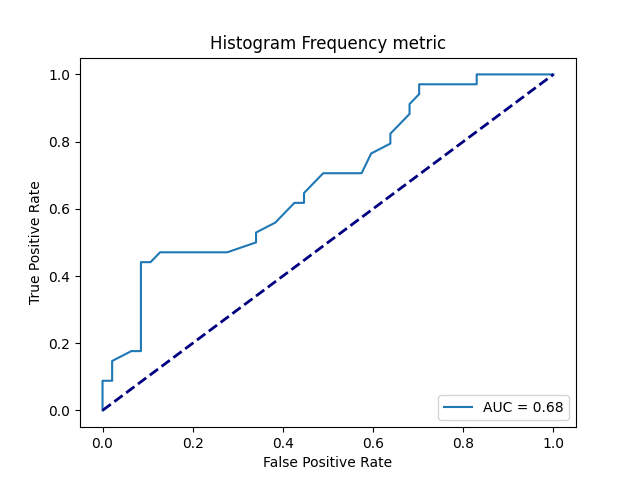
\includegraphics[width=\textwidth]{Figures/BlurredImages/output_HF_roc.png}
        \caption{This metric does not perform very well, however better than random.}
        \label{fig:hf_roc}
    \end{subfigure}
    \begin{subfigure}[t]{0.49\textwidth}
        \centering
        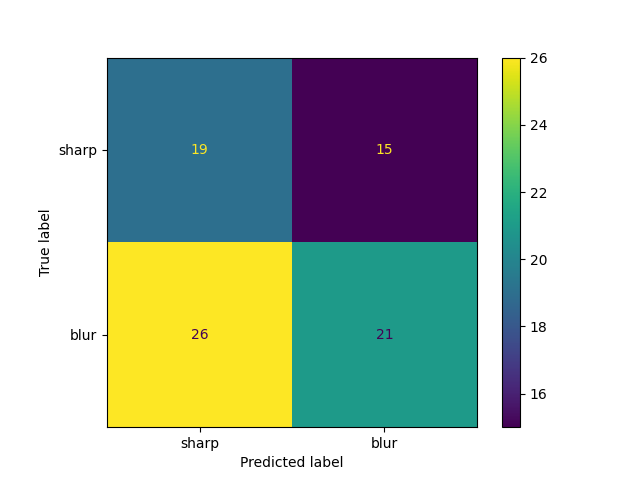
\includegraphics[width=\textwidth]{Figures/BlurredImages/output_FM_conf_mat.png}
        \caption{Many of the blurry images are evaluated as sharp by the FM metric.}
        \label{fig:hf_conf_mat}
    \end{subfigure}
    \hfill
    \begin{subfigure}[t]{0.49\textwidth}
        \centering
        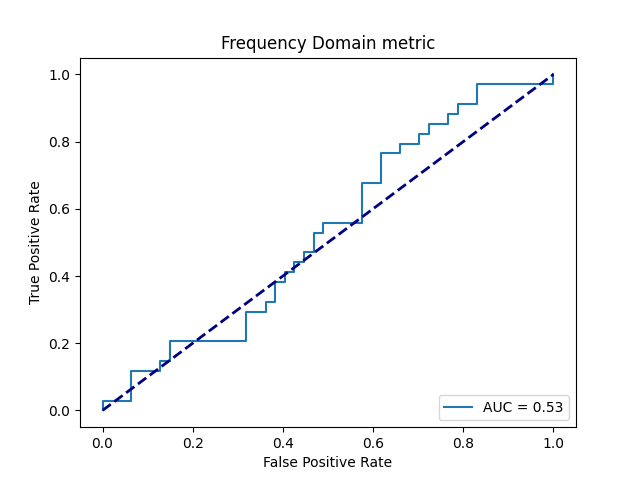
\includegraphics[width=\textwidth]{Figures/BlurredImages/output_FM_roc.png}
        \caption{This metric seems to provide almost random results, that is the metric seems to perform very badly on the current type of images.}
        \label{fig:hf_roc}
    \end{subfigure}
\end{figure}

From the above plots, it is clear that CPBD an HF performs better than FM. These metrics will be combined...
%Specificity/sensitivity on the above results:


\section{Choosing the best metric}
In this section, the four metrics will be given different parameters to make them perform their best.\footnote{\textcolor{red}{rewrite}}

\subsection{Tweaking parameters}
Some of the chosen metrics have constants that can be adjusted to optimize the correctness of the output scores. This concerns the histogram frequency-based and the frequency domain metrics.

The best possible constants have been chosen experimentally, looking at the AUC value of the outputs when running the metric on the training data set. The constants will be chosen between those that provide the highest AUC values on the training data set both including and excluding the Gaussian blurred images.

\subsubsection{FM}
In the frequency domain image blur measure, the threshold $t=\dfrac{M}{1000}$ is experimentally estimated \footnote{\textit{Experimentally it is observed that this particular threshold value gives a fairly accurate sense of image quality}\cite{FM}}. This will also be done in the following, where the constant for division ($1000$) is varied.

\begin{figure}[H]
    \centering
    \begin{subfigure}[t]{0.48\textwidth}
        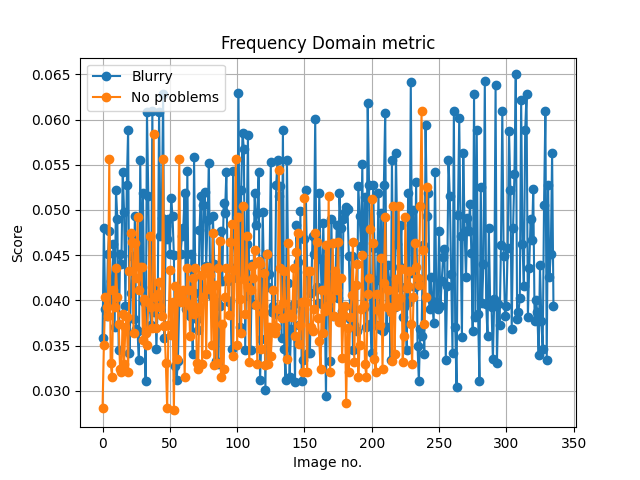
\includegraphics[width=\textwidth]{Figures/BlurredImages/tweakFM/102_output_basic_no_gauss.png}
        \caption{}
        \label{fig:FM_basic_102}
    \end{subfigure}\hspace{1em}
    \begin{subfigure}[t]{0.48\textwidth}
        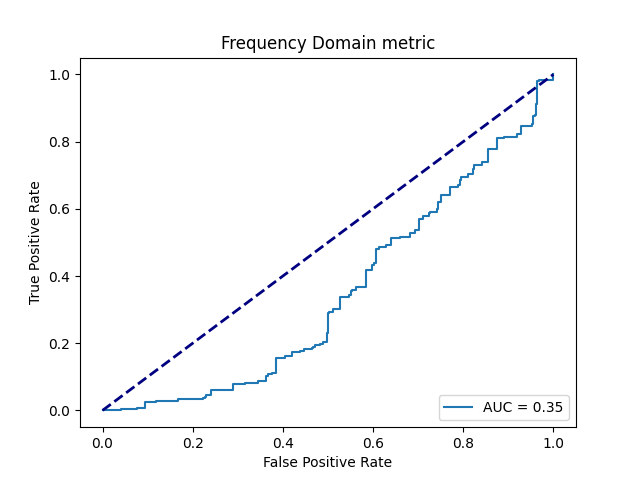
\includegraphics[width=\textwidth]{Figures/BlurredImages/tweakFM/102_output_roc_no_gauss.png}
        \caption{The worst performance with constant $102$ and no Gauss, having AUC$=0.35$.}
        \label{fig:FM_roc_102}
    \end{subfigure}\hspace{1em}
    \begin{subfigure}[t]{0.48\textwidth}
        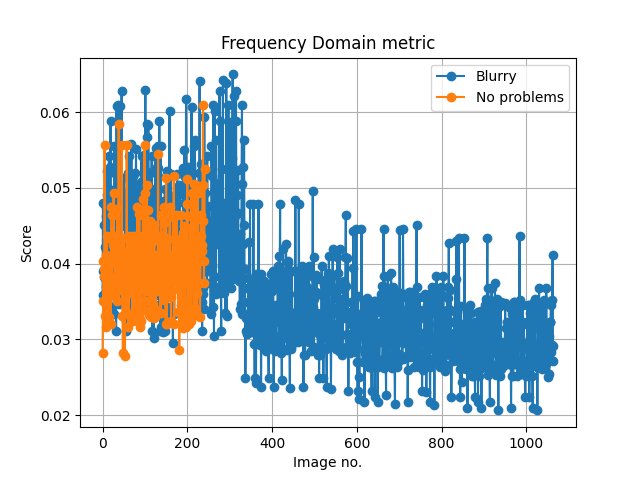
\includegraphics[width=\textwidth]{Figures/BlurredImages/tweakFM/102_output_basic.png}
        \caption{}
        \label{fig:FM_basic_gauss_102}
    \end{subfigure}\hspace{1em}
    \begin{subfigure}[t]{0.48\textwidth}
        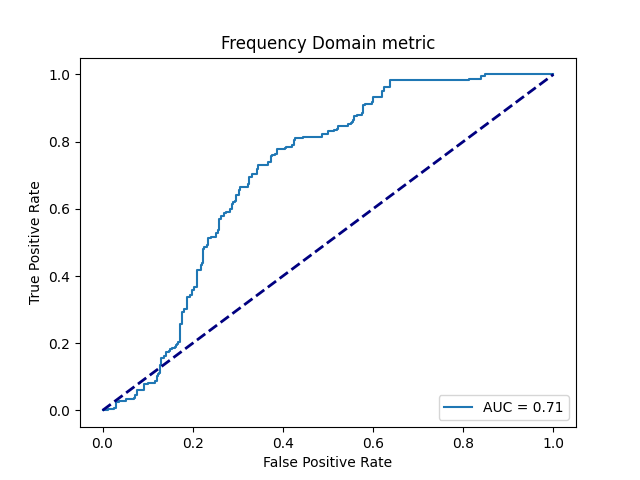
\includegraphics[width=\textwidth]{Figures/BlurredImages/tweakFM/102_output_roc.png}
        \caption{The performance with constant $102$ on the training set including Gauss, having AUC$=0.71$.}
        \label{fig:FM_roc_gauss_102}
    \end{subfigure}
    \caption{The output with a constant of value $102$}
\end{figure}

\begin{figure}[H]
    \begin{subfigure}[t]{0.48\textwidth}
        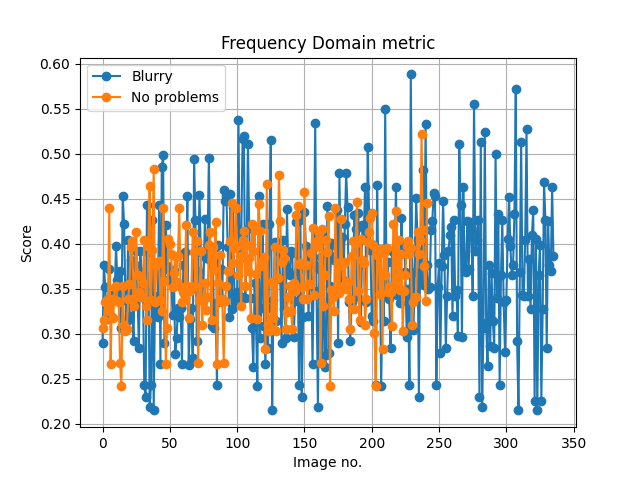
\includegraphics[width=\textwidth]{Figures/BlurredImages/tweakFM/2202_output_basic.png}
        \caption{}
        \label{fig:FM_basic_2202}
    \end{subfigure}\hspace{1em}
    \begin{subfigure}[t]{0.48\textwidth}
        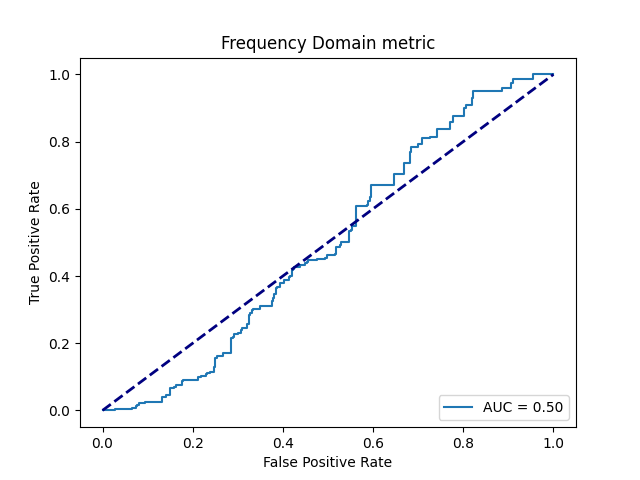
\includegraphics[width=\textwidth]{Figures/BlurredImages/tweakFM/2202_output_roc.png}
        \caption{The AUC$=0.5$ on the training set without Gauss with the constant $2202$.}
        \label{fig:FM_roc_2202}
    \end{subfigure}\hspace{1em}
    \begin{subfigure}[t]{0.48\textwidth}
        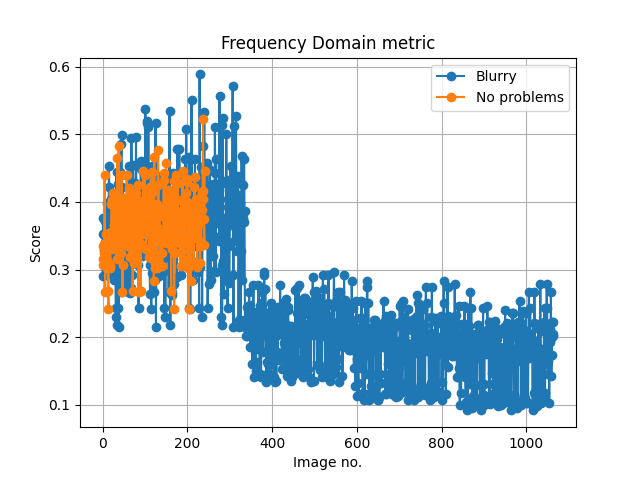
\includegraphics[width=\textwidth]{Figures/BlurredImages/tweakFM/2202_output_basic_gauss.png}
        \caption{}
        \label{fig:FM_basic_gauss_2202}
    \end{subfigure}\hspace{1em}
    \begin{subfigure}[t]{0.48\textwidth}
        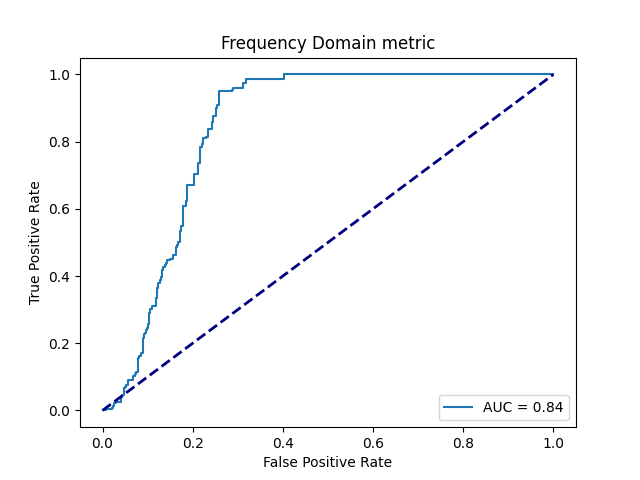
\includegraphics[width=\textwidth]{Figures/BlurredImages/tweakFM/2202_output_roc_gauss.png}
        \caption{One of the best performances with Gauss is with the constant $2202$, having AUC$=0.84$.}
        \label{fig:FM_roc_gauss_2202}
    \end{subfigure}
    \caption{The output with a constant of value $2202$}
\end{figure}
The Gaussian blurred images will not be taking into account when choosing the constant for the metric, as they distort the result. This can be seen in the above images, where the metric performs excellent on the training set including the Gaussian images, while at the same time it performs quite badly on the training set without. The AUC in the tests on the training set without Gauss did not manage to exceed $53\%$, however, the lowest value was $35\%$, which gives an AUC of $100\%-35\%=65\%$. However, doing this, the metric would classify the Gaussian blurred images as sharper when applying more blur.

As this metric performs worst of all 4\textcolor{red}{as can be seen...}, it will not be taken into account in the following sections.

% \subsubsection{CPBD}
% The cumulative probability of blur detection metric has a threshold that classifies a block as smooth if the number of edge pixels in the block is below $0.2\%$ of the pixels in the whole block.
% theta can't be estimated, as we do not have the data for it...
% \textit{In (1), the values of and are chosen, by means of a least-square fitting, to increase the correspondence of (1) with the experimentally determined psychometric function (given by the normalized histogram of the subjects’ responses).\cite{JNB}}

\subsubsection{HF}

\subsection{Metric performance \textcolor{red}{rewrite...}}
Following are statistics on the three metrics.
In the histogram frequency-based metric, the two thresholds, $minDCTValue$ and $maxHistValue$, can be adjusted for optimizing the output.

\begin{figure}[H]
    \centering
    \begin{subfigure}[t]{0.48\textwidth}
        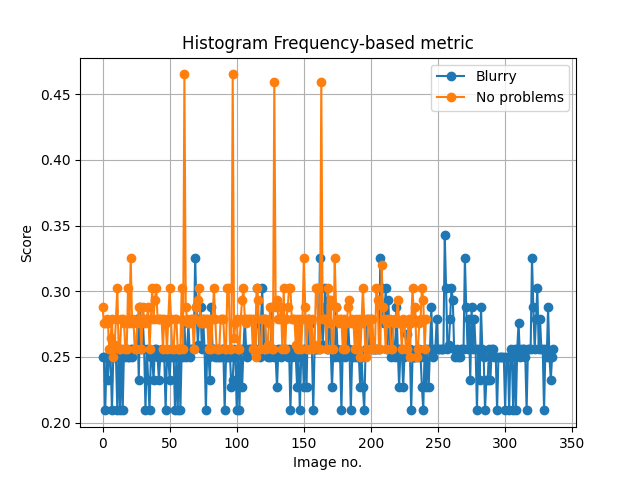
\includegraphics[width=\textwidth]{Figures/BlurredImages/tweakHF/min1_max0.085_output_basic_no_gauss.png}
        \caption{}
        \label{fig:HF_basic_85}
    \end{subfigure}\hspace{1em}
    \begin{subfigure}[t]{0.48\textwidth}
        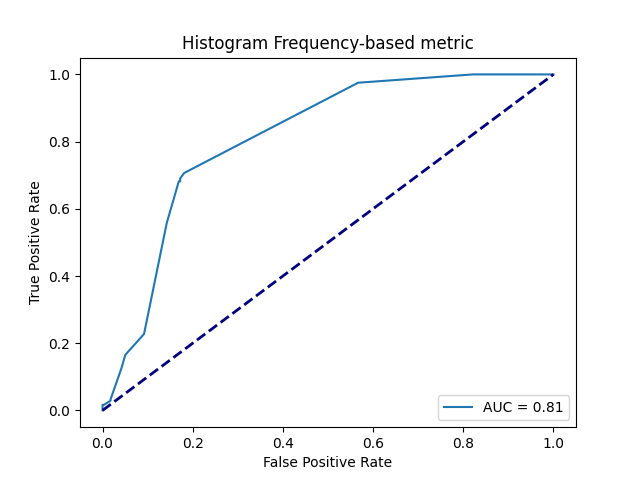
\includegraphics[width=\textwidth]{Figures/BlurredImages/tweakHF/min1_max0.085_output_roc_no_gauss.png}
        \caption{One of the two best performances without Gauss have constants $minDCTValue=1$ and $maxHistValue=0.085$, having AUC$=0.81$.}
        \label{fig:HF_roc_85}
    \end{subfigure}\hspace{1em}
    \begin{subfigure}[t]{0.48\textwidth}
        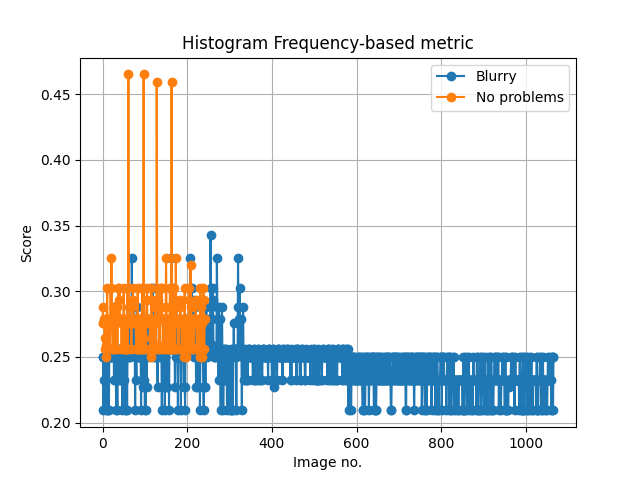
\includegraphics[width=\textwidth]{Figures/BlurredImages/tweakHF/min1_max0.085_output_basic.png}
        \caption{}
        \label{fig:HF_basic_gauss_85}
    \end{subfigure}\hspace{1em}
    \begin{subfigure}[t]{0.48\textwidth}
        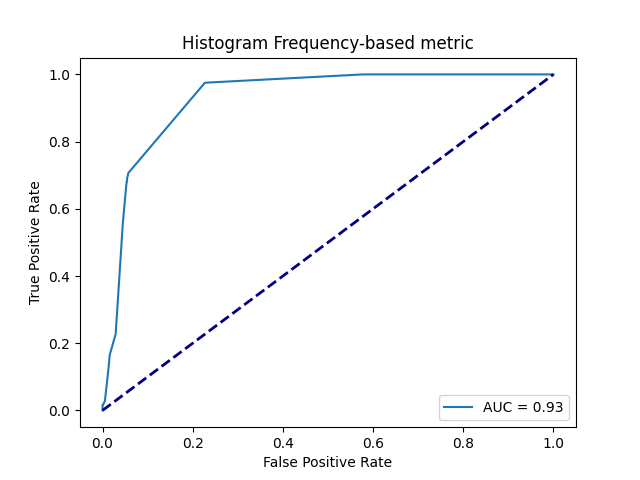
\includegraphics[width=\textwidth]{Figures/BlurredImages/tweakHF/min1_max0.085_output_roc.png}
        \caption{The output on the training set including Gauss on constants $minDCTValue=1$ and $maxHistValue=0.085$, having AUC$=0.93$.}
        \label{fig:HF_roc_gauss_85}
    \end{subfigure}
    \caption{The output with $minDCTValue=1$ and $maxHistValue=0.085$.}
\end{figure}

\begin{figure}[H]
    \begin{subfigure}[t]{0.48\textwidth}
        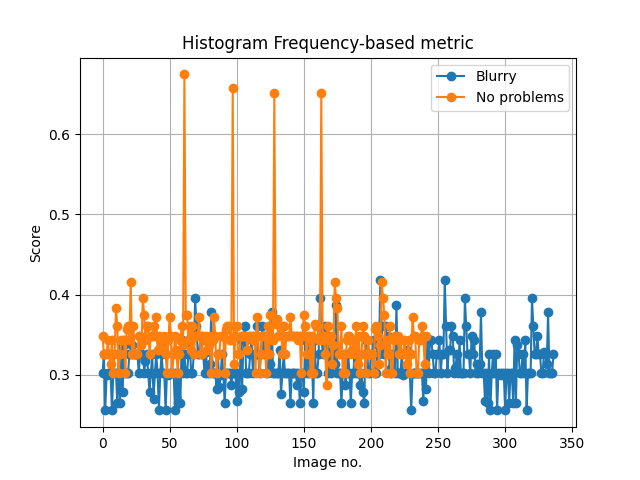
\includegraphics[width=\textwidth]{Figures/BlurredImages/tweakHF/min0_max0.115_output_basic.png}
        \caption{}
        \label{fig:HF_basic_115}
    \end{subfigure}\hspace{1em}
    \begin{subfigure}[t]{0.48\textwidth}
        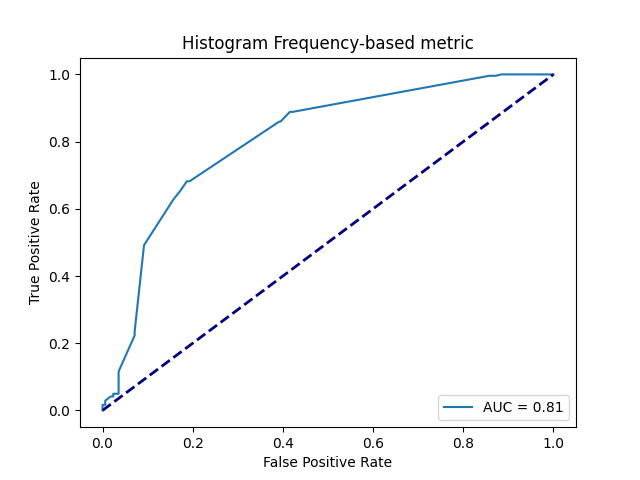
\includegraphics[width=\textwidth]{Figures/BlurredImages/tweakHF/min0_max0.115_output_roc.png}
        \caption{One of the two best performances on the training set with $minDCTValue=0$, $maxHistValue=0.115$ and without Gauss, having AUC$=0.81$.}
        \label{fig:HF_roc_115}
    \end{subfigure}\hspace{1em}
    \begin{subfigure}[t]{0.48\textwidth}
        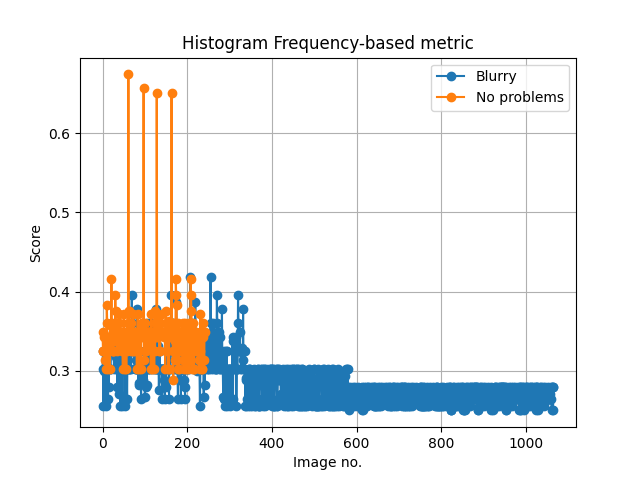
\includegraphics[width=\textwidth]{Figures/BlurredImages/tweakHF/gauss_min0_max0.115_output_basic.png}
        \caption{}
        \label{fig:HF_basic_gauss_115}
    \end{subfigure}\hspace{1em}
    \begin{subfigure}[t]{0.48\textwidth}
        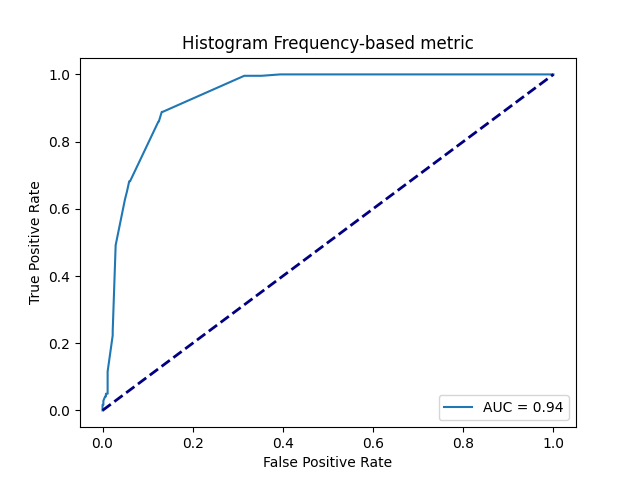
\includegraphics[width=\textwidth]{Figures/BlurredImages/tweakHF/gauss_min0_max0.115_output_roc.png}
        \caption{The best performance with Gauss is with $minDCTValue=0$ and $maxHistValue=0.115$, having AUC$=0.94$.}
        \label{fig:HF_roc_gauss_115}
    \end{subfigure}
    \caption{The output with $minDCTValue=0$ and $maxHistValue=0.115$.}
    \label{fig:tweakHF}
\end{figure}
The correctness of the output of the algorithm doesn't seem to be distorted by the Gaussian blurred images. In figure \ref{fig:tweakHF} the ROC curves with highest scores are displayed. As can be seen, the output of running the algorithm on the training set without Gaussian blurred images performs very well in two different situations. The correctness is also very high and almost identical for the results including the Gaussian blurred images. However, it is a little better with the lower $minDCTValue=0$, whose purpose is filtering away noise. That is, when no noise is filtered away.

Knowing this, the $minDCTValue=1$ and $maxHistValue=0.085$ are chosen for the metric, as the purpose of the metric is not detecting Gaussian blur, but blur in non-manipulated images, where noise could occur, and as the worsening of the results on the Gaussian blurred images is insignificant.

%The Gaussian blurred images will not be used for training the metrics, as they distort the results. This can be seen in the above images, where the metric tend to perform excellent on the the training set including the Gaussian images, but not very well on the training set without. On the other hand, the metric performs well when given other parameters and the training set without Gauss.


\subsubsection{Histogram frequency-based metric}
\begin{figure}[H]
    \centering
    \begin{subfigure}[t]{0.48\textwidth}
        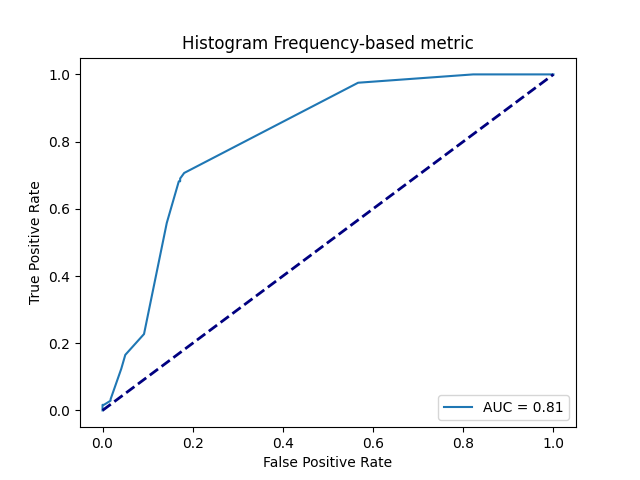
\includegraphics[width=\textwidth]{Figures/BlurredImages/results_on_thresholds/output_roc_hf.png}
        \caption{}
        \label{fig:HF_roc}
    \end{subfigure}\hspace{1em}
    \begin{subfigure}[t]{0.48\textwidth}
        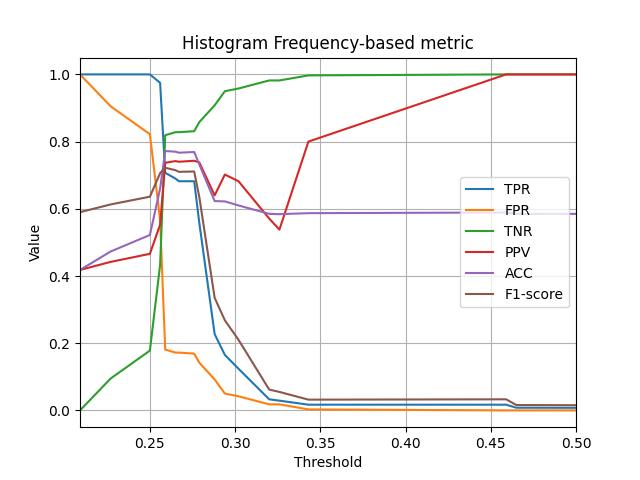
\includegraphics[width=\textwidth]{Figures/BlurredImages/results_on_thresholds/threshold_test_scores_hf.png}
        \caption{}
        \label{fig:HF_thresh}
    \end{subfigure}\hspace{1em}
    \begin{subfigure}[t]{0.48\textwidth}
        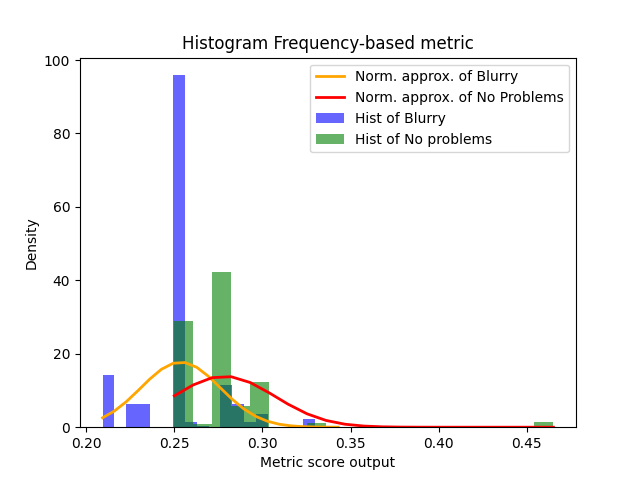
\includegraphics[width=\textwidth]{Figures/BlurredImages/results_on_thresholds/output_dens_hf.png}
        \caption{}
        \label{fig:HF_dens}
    \end{subfigure}\hspace{1em}
    \caption{}
    \label{fig:HF_final}
\end{figure}

\subsection{Best version of other metrics...}

\subsubsection{CPBD}
\begin{figure}[H]
    \centering
    \begin{subfigure}[t]{0.48\textwidth}
        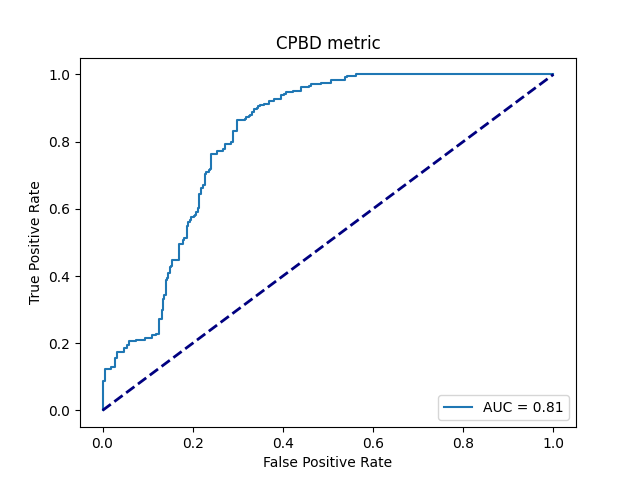
\includegraphics[width=\textwidth]{Figures/BlurredImages/results_on_thresholds/output_roc_cpbd.png}
        \caption{}
        \label{fig:CPBD_roc}
    \end{subfigure}\hspace{1em}
    \begin{subfigure}[t]{0.48\textwidth}
        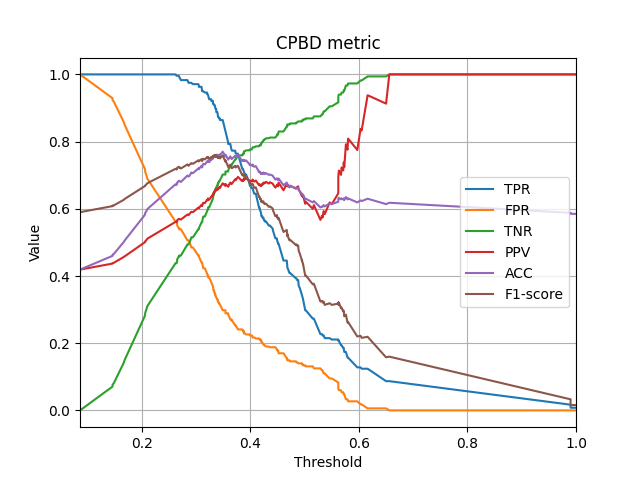
\includegraphics[width=\textwidth]{Figures/BlurredImages/results_on_thresholds/threshold_test_scores_cpbd.png}
        \caption{}
        \label{fig:CPBD_thresh}
    \end{subfigure}\hspace{1em}
    \begin{subfigure}[t]{0.48\textwidth}
        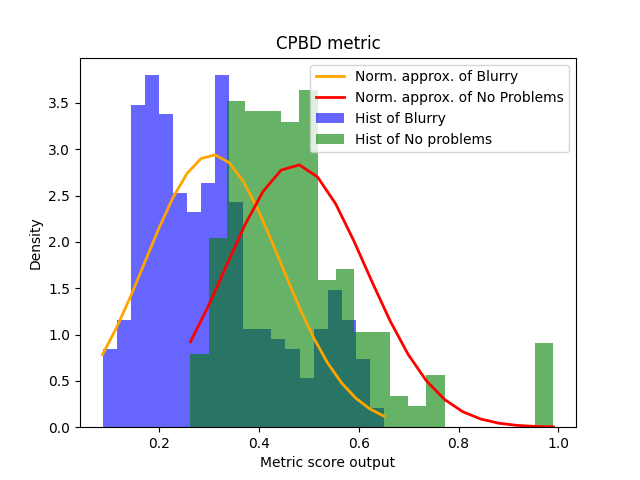
\includegraphics[width=\textwidth]{Figures/BlurredImages/results_on_thresholds/output_dens_cpbd.png}
        \caption{}
        \label{fig:CPBD_dens}
    \end{subfigure}\hspace{1em}
    \caption{}
    \label{fig:CPBD_final}
\end{figure}

\subsubsection{Variance of Laplacian}
\textbf{JPG}\\

\begin{figure}[H]
    \centering
    \begin{subfigure}[t]{0.48\textwidth}
        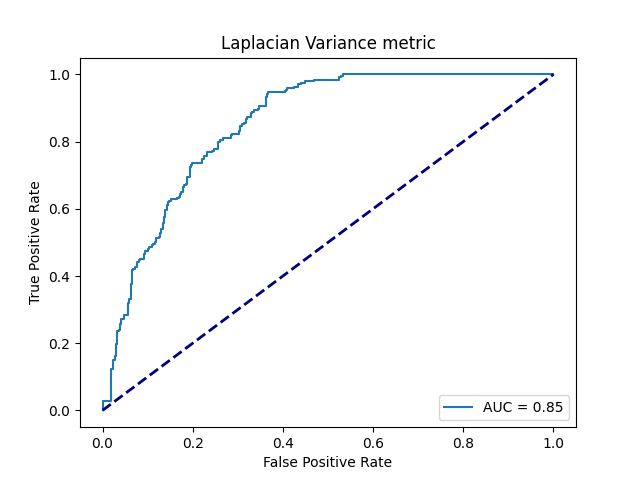
\includegraphics[width=\textwidth]{Figures/BlurredImages/results_on_thresholds/output_roc_lv.png}
        \caption{}
        \label{fig:LV_roc}
    \end{subfigure}\hspace{1em}
    \begin{subfigure}[t]{0.48\textwidth}
        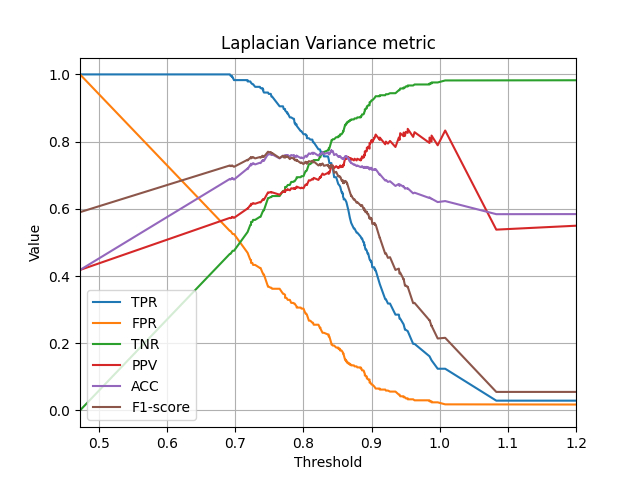
\includegraphics[width=\textwidth]{Figures/BlurredImages/results_on_thresholds/threshold_test_scores_lv.png}
        \caption{}
        \label{fig:LV_thresh}
    \end{subfigure}\hspace{1em}
    \begin{subfigure}[t]{0.48\textwidth}
        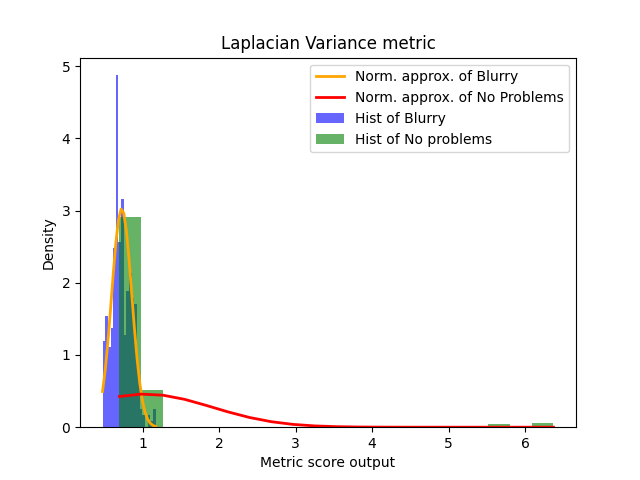
\includegraphics[width=\textwidth]{Figures/BlurredImages/results_on_thresholds/output_dens_lv.png}
        \caption{}
        \label{fig:LV_dens}
    \end{subfigure}\hspace{1em}
    \caption{}
    \label{fig:LV_final}
\end{figure}

\textbf{PNG}

\textbf{Outlier}\\
\begin{figure}[H]
    \centering
    \begin{subfigure}[t]{0.6\textwidth}
        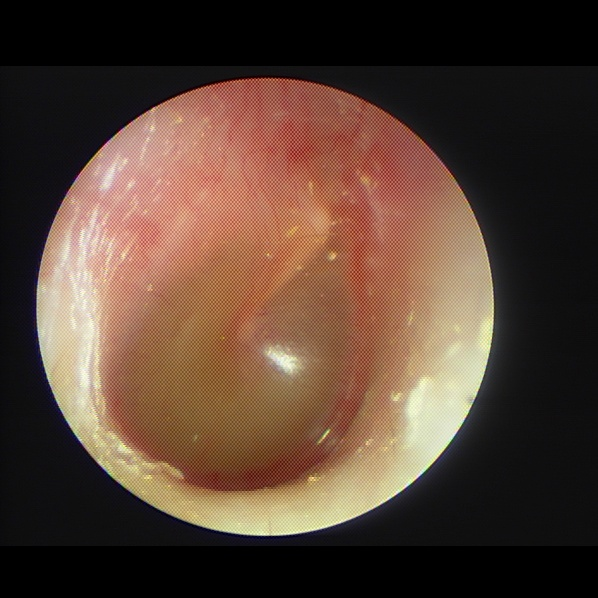
\includegraphics[width=\textwidth]{Figures/BlurredImages/lv/33.png}
        \caption{This image recieves a score of 5.7, whereas most of the sharp images scores around 1. By looking closely at the image, one can see a grid-like structure on the image pixels, which explains the output in figure \ref{fig:LV_very_sharp}. \textcolor{red}{add to bilag}}
  %      \label{fig:LV_roc}
    \end{subfigure}\hspace{1em}
    \begin{subfigure}[t]{0.6\textwidth}
        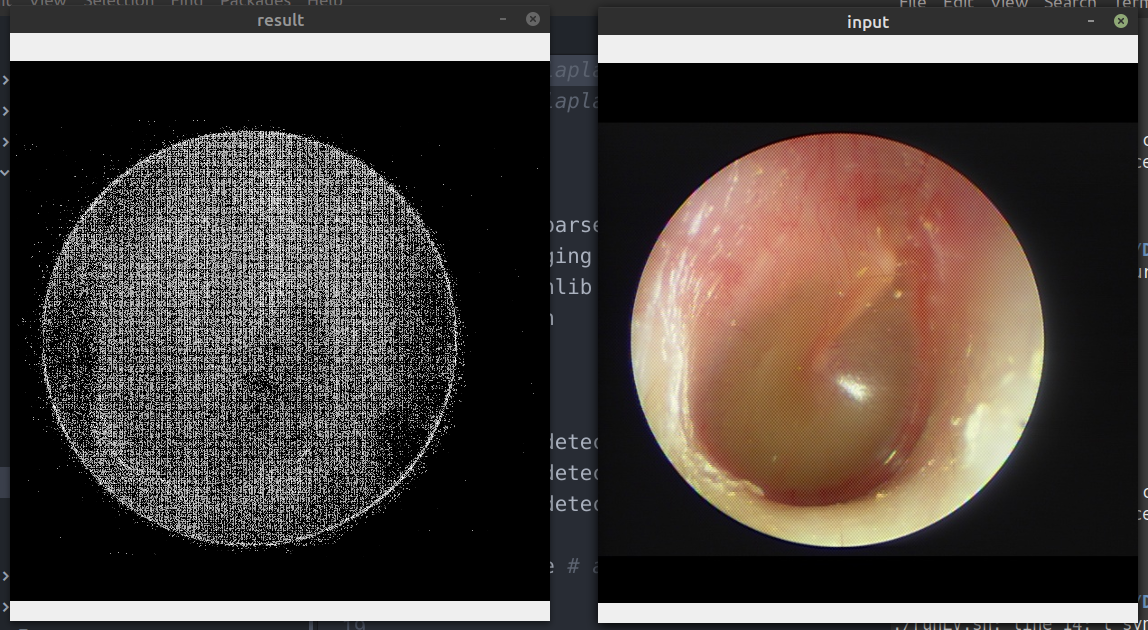
\includegraphics[width=\textwidth]{Figures/BlurredImages/lv/lv_very_sharp.png}
        \caption{}
        \label{fig:LV_very_sharp}
    \end{subfigure}\hspace{1em}
    \caption{}
    \begin{subfigure}[t]{0.6\textwidth}
        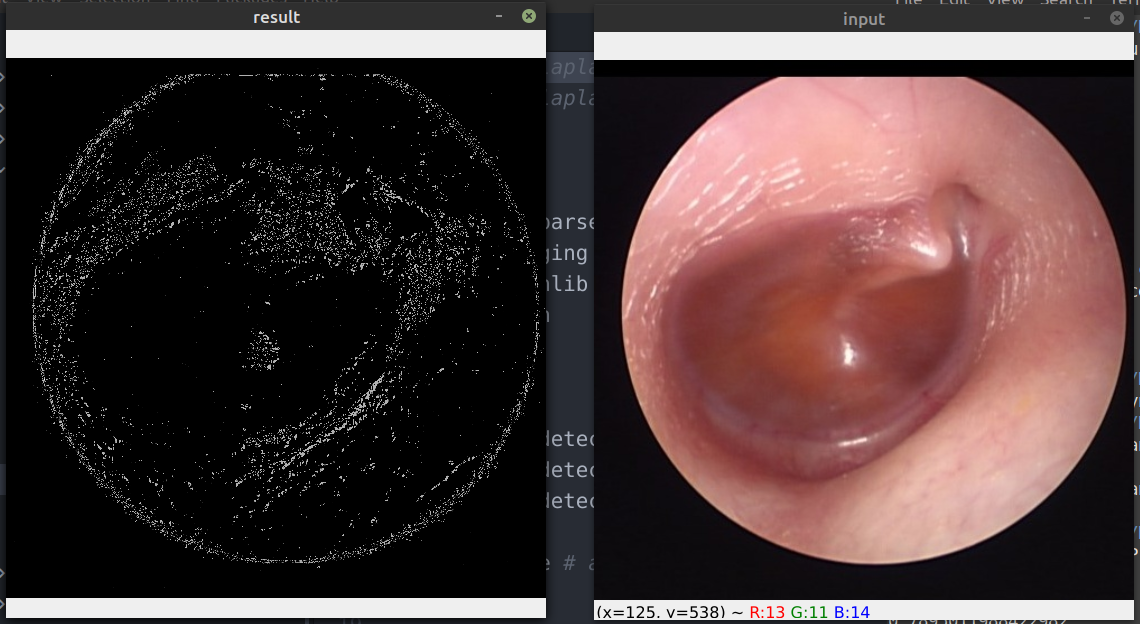
\includegraphics[width=\textwidth]{Figures/BlurredImages/lv/lv_normal.png}
        \caption{}
 %       \label{fig:LV_thresh}
    \end{subfigure}\hspace{1em}
%    \label{fig:LV_final}
\end{figure}




\subsection{Combining the metrics}
The three metrics, CPBD, Variance of Lapracian and Histogram Frequency-based metric, will be combined to form 4 new metrics. This is done by combining the outputs of the metrics as $m_{new}=\alpha \cdot m1 + (1-\alpha) \cdot m2$, where $m1$ and $m2$ are two different metrics.


\subsubsection{Merge of CPBD and Variance of Laplacian}
\textbf{Highest AUC = 90\%}
\begin{figure}[H]
    \centering
    \begin{subfigure}[t]{0.48\textwidth}
        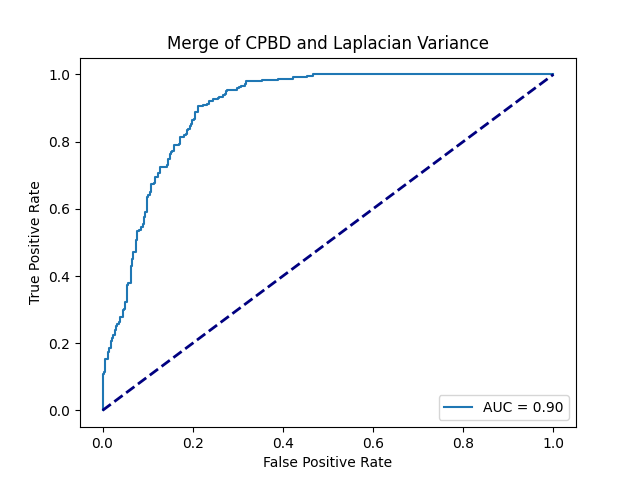
\includegraphics[width=\textwidth]{Figures/BlurredImages/results_on_thresholds/output_roc_cpbd_lv.png}
        \caption{}
        \label{fig:CPBD_LV_roc}
    \end{subfigure}\hspace{1em}
    \begin{subfigure}[t]{0.48\textwidth}
        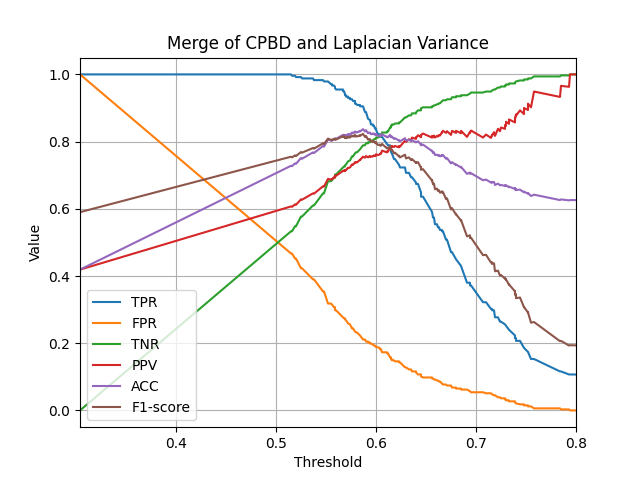
\includegraphics[width=\textwidth]{Figures/BlurredImages/results_on_thresholds/threshold_test_scores_cpbd_lv.png}
        \caption{}
        \label{fig:CPBD_LV_thresh}
    \end{subfigure}\hspace{1em}
    \begin{subfigure}[t]{0.48\textwidth}
        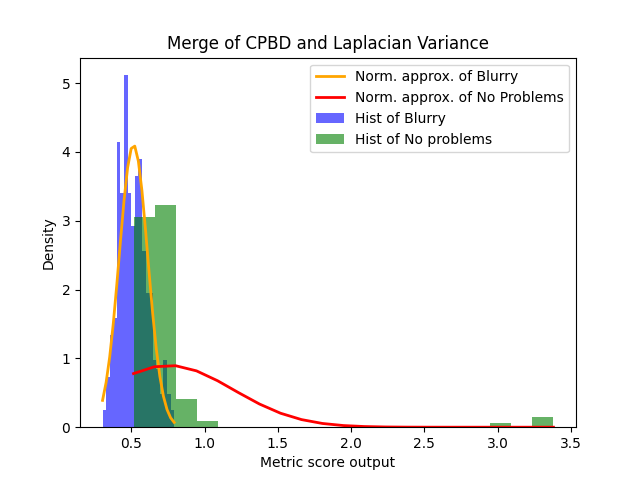
\includegraphics[width=\textwidth]{Figures/BlurredImages/results_on_thresholds/output_dens_cpbd_lv.png}
        \caption{}
        \label{fig:CPBD_LV_dens}
    \end{subfigure}\hspace{1em}
    \caption{}
    \label{fig:CPBD_LV_final}
\end{figure}

\subsubsection{Merge of CPBD and Histogram frequency-based metric}
\begin{figure}[H]
    \centering
    \begin{subfigure}[t]{0.48\textwidth}
        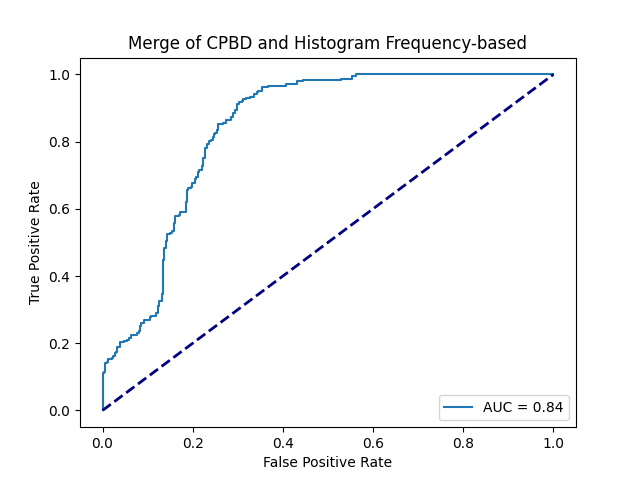
\includegraphics[width=\textwidth]{Figures/BlurredImages/results_on_thresholds/output_roc_cpbd_hf.png}
        \caption{}
        \label{fig:CPBD_HF_roc}
    \end{subfigure}\hspace{1em}
    \begin{subfigure}[t]{0.48\textwidth}
        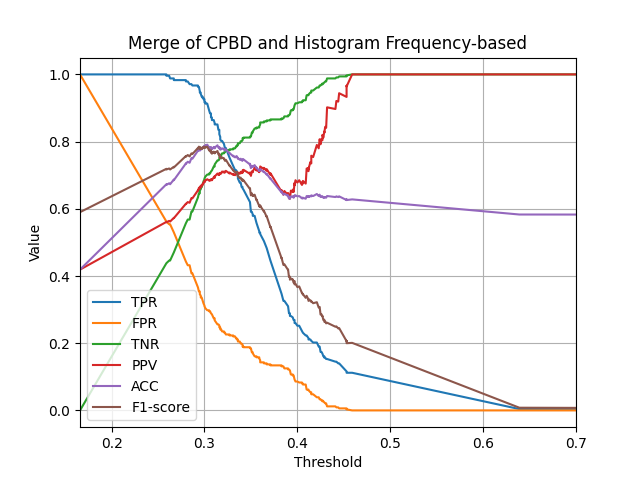
\includegraphics[width=\textwidth]{Figures/BlurredImages/results_on_thresholds/threshold_test_scores_cpbd_hf.png}
        \caption{}
        \label{fig:CPBD_HF_thresh}
    \end{subfigure}\hspace{1em}
    \begin{subfigure}[t]{0.48\textwidth}
        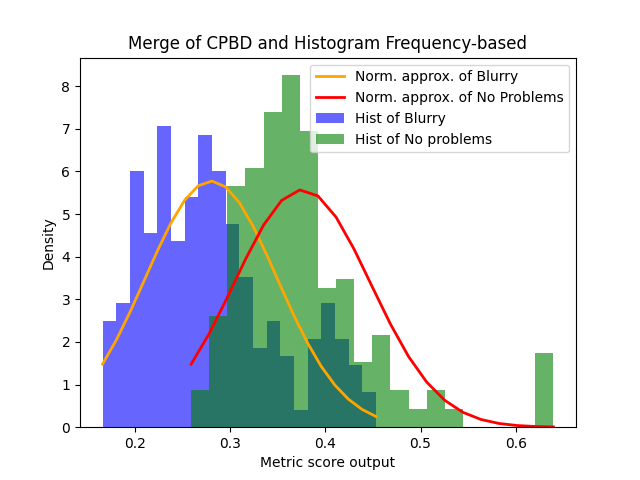
\includegraphics[width=\textwidth]{Figures/BlurredImages/results_on_thresholds/output_dens_cpbd_hf.png}
        \caption{}
        \label{fig:CPBD_HF_dens}
    \end{subfigure}\hspace{1em}
    \caption{}
    \label{fig:CPBD_HF_final}
\end{figure}

\subsubsection{Merge of Histogram frequency-based metric and Variance of Laplacian}
\begin{figure}[H]
    \centering
    \begin{subfigure}[t]{0.48\textwidth}
        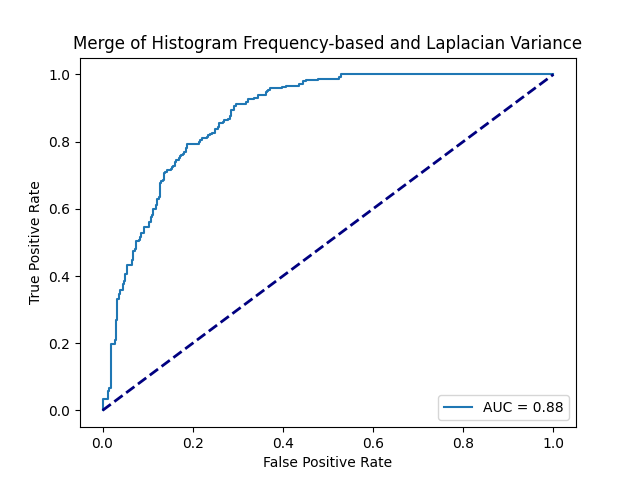
\includegraphics[width=\textwidth]{Figures/BlurredImages/results_on_thresholds/output_roc_hf_lv.png}
        \caption{}
        \label{fig:HF_LV_roc}
    \end{subfigure}\hspace{1em}
    \begin{subfigure}[t]{0.48\textwidth}
        \includegraphics[width=\textwidth]{Figures/BlurredImages/results_on_thresholds/threshold_test_scores_hf_lv.png}
        \caption{}
        \label{fig:HF_LV_thresh}
    \end{subfigure}\hspace{1em}
    \begin{subfigure}[t]{0.48\textwidth}
        \includegraphics[width=\textwidth]{Figures/BlurredImages/results_on_thresholds/output_dens_hf_lv.png}
        \caption{}
        \label{fig:HF_LV_dens}
    \end{subfigure}\hspace{1em}
    \caption{}
    \label{fig:HF_LV_final}
\end{figure}

\subsubsection{Merge of CPBD, Histogram frequency-based metric and Variance of Laplacian}
\begin{figure}[H]
    \centering
    \begin{subfigure}[t]{0.48\textwidth}
        \includegraphics[width=\textwidth]{Figures/BlurredImages/results_on_thresholds/output_roc_cpbd_hf_lv.png}
        \caption{}
        \label{fig:CPBD_HF_LV_roc}
    \end{subfigure}\hspace{1em}
    \begin{subfigure}[t]{0.48\textwidth}
        \includegraphics[width=\textwidth]{Figures/BlurredImages/results_on_thresholds/threshold_test_scores_cpbd_hf_lv.png}
        \caption{}
        \label{fig:CPBD_HF_LV_thresh}
    \end{subfigure}\hspace{1em}
    \begin{subfigure}[t]{0.48\textwidth}
        \includegraphics[width=\textwidth]{Figures/BlurredImages/results_on_thresholds/output_dens_cpbd_hf_lv.png}
        \caption{}
        \label{fig:CPBD_HF_LV_dens}
    \end{subfigure}\hspace{1em}
    \caption{}
    \label{fig:CPBD_HF_LV_final}
\end{figure}



\subsection{"Training" the metrics}
The goal is to avoid false positives (\textbf{FP}: classified as sharp when blurry), as far as possible, as these can distort the results from the data later on, while still achieving some positive outputs.

\textbf{Choosing the threshold:}\\
Let the user choose an acceptable TNR (specificity), e.g. 98\%.\\
After this, find the corresponding threshold and choose the metric with the highest accuracy, as it will provide a possibility that some images will be "accepted", that is, classified as sharp. 

We could also calculate summed distance, d, of some rates... TPR (sensitivity), F1-score, precision...  to the top and bottom border (1 and 0) according to which border is desired for that particular rate. Then choose the metric with smallest d.


\begin{itemize}
    % \item minimize FPR (sharp when not) ($1-TNR$)
    \item maximize TNR (how many are blurry when blurry)
    \item maximize TPR (we would still like some possibility that images are classified "sharp")
    \item maximize PPV (part declared sharp when sharp)
    \item high f1-score for general score + do not produce FP (to not filter away too many negatives)
\end{itemize}


The following graphs displays output on the training data set excluding the Gaussian blurred images.



